\chapter{Achimate -ADM}

El método ADM y en general el marco TOGAF realiza el análisis arquitectónico con alto nivel de abstracción para visualizar, detectar y
	documentar oportunidades y riesgos durante el desarrollo de la arquitectura, direccionando la arquitectura empresarial con la ayuda de sus herramientas.
TOGAF esta compuesto por 3 partes principales el método de desarrollo ADM (Architecture Development Method), la taxonomía empresarial (Enterprise Continuum) y la base de recursos (Architecture Repository). Aborda el desarrollo a partir de 4 niveles de abstracción:
\begin{itemize}
	\item Arquitectura de Negocio
	\item Arquitectura de Aplicación
	\item Arquitectura de Datos
	\item Arquitectura Tecnológica
\end{itemize}
ADM muestra estos niveles de abstracción en diferentes fases que determinan la linea base (baseline) y el final del nivel de abstracción (target), donde el analisis de brecha (gap analysis - figura 5.1) permite conocer el estado final de la arquitectura despues de una o varias iteraciones.
\begin{figure}[H]
	\centering
	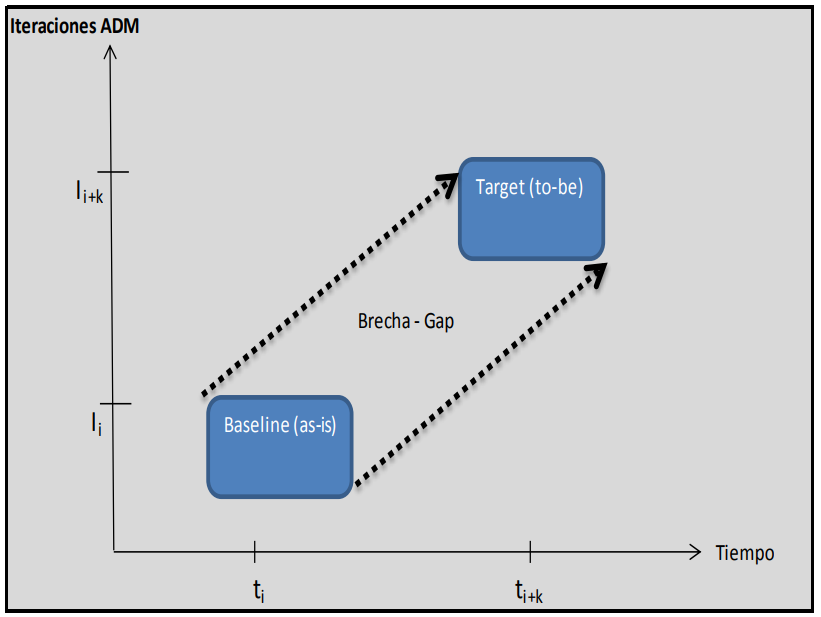
\includegraphics[width=1.0\textwidth]{imagenes/Captura.PNG}
	\caption{Analisis de Brecha -Iteraciones ADM}
	\label{fig:gap_analysis}
\end{figure}

Este análisis mide los objetivos de arquitectura y el grado de la madurez alcanzados por la organización

ADM consta de 8  niveles o etapas y un paso preliminar donde se describen las actividades iniciales, principios y capacidades de la arquitectura objetivo, también se realiza una adaptación del marco de trabajo para ajustarlo a las necesidades de la organización.
\cite{FGuti}

\begin{figure}[H]
	\centering
	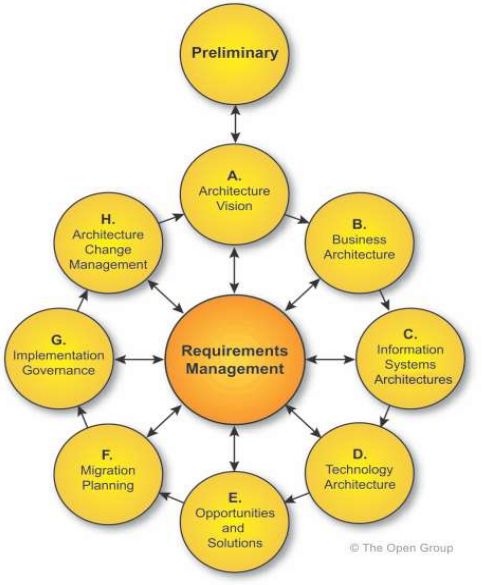
\includegraphics[width=1.0\textwidth]{imagenes/Captura1.PNG}
	\caption{Etapas del Método ADM}
	\label{fig:gap_analysis}
\end{figure}

Las primeras cuatro fases definen los niveles de abstracción antes mencionados para el desarrollo de la arquitectura, la fase E de la interacción define oportunidades y soluciones que se deben implementar.

Estas oportunidades y soluciones se identifican e incluyen en el plan de migración, fase F. En esta fase se desarrolla el producto de software con los requerimientos y especificaciones obtenidos de las anteriores fases, luego lleva a su implementación (fase G) y como finalidad lleva la arquitectura de un estado base (baseline) al estado objetivo (target), estas dos fases dan gobernabilidad y gestión de control de cambios a la arquitectura. Este ciclo se repite hasta llegar a la vision establecida en la fase preliminar junto con la vision inicialmente concebida.


\section{TOGAF}
\subsection{Resumen: capa de negocio}

\begin{center}
	\begin{longtable}[H]{|p{5cm}|p{6cm}|p{3cm}|}
		\hline
		\textbf{Concepto} &  \centering \textbf{Definición} & \textbf{Notación} \\
		\hline
		\endfirsthead
		
		
		\hline
		\textbf{Concepto} &  \centering \textbf{Definición} & \textbf{Notación} \\
		\hline
		\endhead
		
		%inicio contenido tabla 
		
		\centering \textbf{Actor de negocio}\\ \textbf{(Business actor)} & Una entidad organizativa que es capaz de realizar el comportamiento.         & 
		\raisebox{-\totalheight}{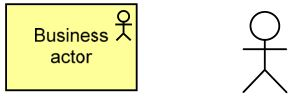
\includegraphics[scale=0.36]{imagenes/lenguaje/Bussines/actor}}\\ 		\hline         
		
		
		\centering \textbf{Papel del negocio}\\ \textbf{(Business role)} & La responsabilidad de realizar un comportamiento específico, al cual un actor puede ser asignado.&\raisebox{-\totalheight}{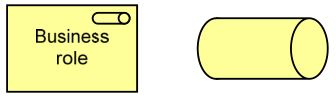
\includegraphics[scale=0.36,]{imagenes/lenguaje/Bussines/role}}\\
		\hline
		
		
		\centering \textbf{Colaboración Empresarial}\\ \textbf{(Business Collaboration)} & Un agregado de dos o más funciones empresariales que trabajan juntas para realizar un comportamiento colectivo. &  \raisebox{-\totalheight}{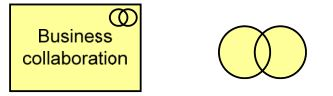
\includegraphics[scale=0.36,] {imagenes/lenguaje/Bussines/collaboration}}\\ 
		\hline
		
		
		\centering \textbf{Interfaz de negocios}\\ \textbf{(Business interface)} & Un punto de acceso donde un servicio comercial está disponible para el medio ambiente..&  \raisebox{-\totalheight}{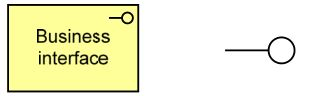
\includegraphics[scale=0.36,]{imagenes/lenguaje/Bussines/interface}}\\ 
		\hline
		
		\centering \textbf{Ubicación}\\ \textbf{(Location)}& Un punto conceptual o extensión en el espacio.&  
		\raisebox{-\totalheight}{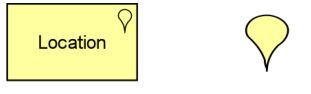
\includegraphics[scale=0.36,]{imagenes/lenguaje/Bussines/location}}\\ 
		\hline
		
		\centering \textbf{Objeto de negocio}\\ \textbf{(Business Object)}& Un elemento pasivo que tiene relevancia desde una perspectiva empresarial.&  
		\raisebox{-\totalheight}{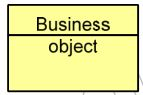
\includegraphics[scale=0.36,]{imagenes/lenguaje/Bussines/object}}\\ 
		\hline
		
		\centering \textbf{Proceso de negocio}\\ \textbf{(Business Process)}& Un elemento de comportamiento que agrupa el comportamiento basado en un ordenamiento de actividades. Se pretende producir un conjunto definido de productos o servicios empresariales.&  
		\raisebox{-\totalheight}{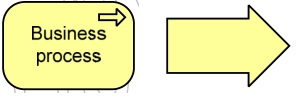
\includegraphics[scale=0.36,]{imagenes/lenguaje/Bussines/process}}\\ 
		\hline
		
		\centering \textbf{Función de negocio}\\ \textbf{(Business Function)}& Un elemento de comportamiento que agrupa el comportamiento basado en un conjunto seleccionado de criterios (normalmente requeridos por los recursos empresariales y / o las competencias).&  
		\raisebox{-\totalheight}{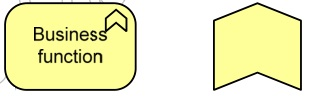
\includegraphics[scale=0.36,]{imagenes/lenguaje/Bussines/funtion}}\\ 
		\hline
		
		\centering \textbf{Interacción de negocios}\\ \textbf{(Business Interaction)}& Un elemento de comportamiento que describe el comportamiento de una colaboración comercial.&  
		\raisebox{-\totalheight}{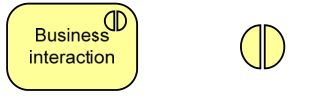
\includegraphics[scale=0.36,]{imagenes/lenguaje/Bussines/interaction}}\\ 
		\hline
		
		\centering \textbf{Evento de negocios}\\ \textbf{(Business Event)}& Algo que sucede (internamente o externamente) e influye en el comportamiento.&  
		\raisebox{-\totalheight}{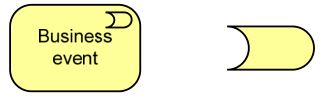
\includegraphics[scale=0.36,]{imagenes/lenguaje/Bussines/event}}\\ 
		\hline
		
		\centering \textbf{Servicio de negocio o empresarial}\\ \textbf{(Business Service)}& Un servicio que satisface una necesidad de negocio para un cliente (interno o externo a la organización).&  
		\raisebox{-\totalheight}{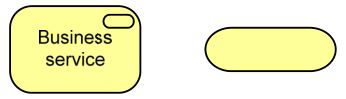
\includegraphics[scale=0.36,]{imagenes/lenguaje/Bussines/service}}\\ 
		\hline
		
		\centering \textbf{Representación}\\ \textbf{(Representation)}& Una forma perceptible de la información transportada por un objeto de negocio.&  
		\raisebox{-\totalheight}{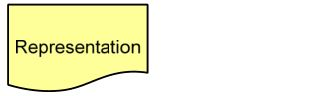
\includegraphics[scale=0.36,]{imagenes/lenguaje/Bussines/representation}}\\ 
		\hline
		
		\centering \textbf{Significado}\\ \textbf{(Meaning)}& Los conocimientos o experiencia presentes en un objeto de negocio o su representación, dado un contexto particular.&  
		\raisebox{-\totalheight}{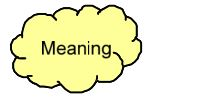
\includegraphics[scale=0.36,]{imagenes/lenguaje/Bussines/meaning}}\\ 
		\hline
		
		\centering \textbf{Valor}\\ \textbf{(Value)}& El valor relativo, la utilidad o la importancia de un servicio o producto comercial.&  
		\raisebox{-\totalheight}{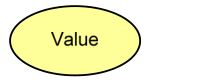
\includegraphics[scale=0.36,]{imagenes/lenguaje/Bussines/value}}\\ 
		\hline
		
		
		\centering \textbf{Producto}\\ \textbf{(Product)}& Un conjunto coherente de servicios, acompañado de un contrato / conjunto de acuerdos, que se ofrece en su conjunto a clientes (internos o externos).&  
		\raisebox{-\totalheight}{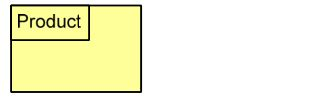
\includegraphics[scale=0.36,]{imagenes/lenguaje/Bussines/product}}\\ 
		\hline
		
		
		\centering \textbf{Contrato}\\ \textbf{(Contract)}& Una especificación formal o informal de acuerdo que especifica los derechos y obligaciones asociados con un producto.&  
		\raisebox{-\totalheight}{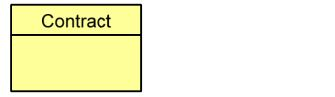
\includegraphics[scale=0.36,]{imagenes/lenguaje/Bussines/contract}}\\ 
		\hline
		
		\caption{Capa de Negocio}
		\label{capa-business}
	\end{longtable}
\end{center}

\subsection{Resumen: capa de aplicación}
\begin{table}[H]
	\centering
	\begin{tabular}{|p{5cm}|p{6cm}|p{3.3cm}|}
		\hline
		\textbf{Concepto}                                                           & \multicolumn{1}{c|}{\textbf{Definición}}                                                             & \textbf{Notación} \\ \hline
		\begin{tabular}[c]{@{}c@{}}\textbf{Componente de Aplicación}\\ \textbf{(Application Component)}\end{tabular} & Una parte modular, desplegable y reemplazable de un sistema de software que encapsula su comportamiento y datos y los expone a través de un conjunto de interfaces.    & 	\raisebox{-\totalheight}{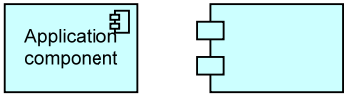
\includegraphics[scale=0.36,]{imagenes/lenguaje/Aplication/componentApp}}
		\\ \hline
		\begin{tabular}[c]{@{}c@{}}\textbf{Colaboración de Aplicación}\\ \textbf{(Application
				collaboration)}\end{tabular}            & 
		Un agregado de dos o más componentes de aplicación que trabajan juntos para realizar un comportamiento colectivo.                         & 
		\raisebox{-0,63\totalheight}{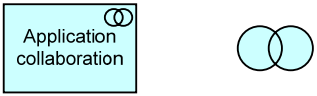
\includegraphics[scale=0.28,]{imagenes/lenguaje/Aplication/collaborationApp}}   \\ \hline
		\begin{tabular}[c]{@{}c@{}}\textbf{Interfaz de Aplicación}\\ \textbf{(Application interface)}\end{tabular}                  & Un punto de acceso donde un servicio de aplicación está disponible para un usuario u otro componente de aplicación &  \raisebox{-0,63\totalheight}{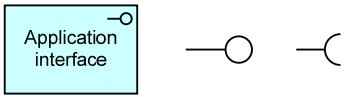
\includegraphics[scale=0.36,]{imagenes/lenguaje/Aplication/interfaceApp}} 
		\\ \hline
		\begin{tabular}[c]{@{}c@{}}\textbf{Objeto de Datos}\\ \textbf{(Data Object)}\end{tabular}                      & Un elemento pasivo adecuado para el procesamiento automatizado.                                  & 
		\raisebox{-0,63\totalheight}{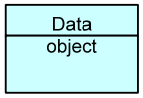
\includegraphics[scale=0.36,]{imagenes/lenguaje/Aplication/dataObjectApp}}
		\\ \hline
		\begin{tabular}[c]{@{}c@{}}\textbf{Función de Aplicación}\\ \textbf{(Function Application)}\end{tabular}                      & 
		Un elemento de comportamiento que agrupa el comportamiento automatizado que puede ser realizado por un componente de aplicación.                                & \raisebox{-0,63\totalheight}{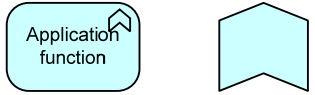
\includegraphics[scale=0.36,]{imagenes/lenguaje/Aplication/functionApp}}
		\\ \hline
		\begin{tabular}[c]{@{}c@{}}\textbf{Interacción de Aplicación}\\ \textbf{(Application
				interaction)}\end{tabular}                      & 
		Un elemento de comportamiento que describe el comportamiento de una colaboración de aplicación                                  & 
		\raisebox{-0,63\totalheight}{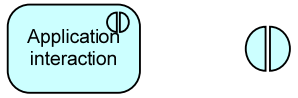
\includegraphics[scale=0.36,]{imagenes/lenguaje/Aplication/interactionApp}}
		\\ \hline
		\begin{tabular}[c]{@{}c@{}}\textbf{Servicio de Aplicación}\\ \textbf{(Application
				Service)}\end{tabular}                      & 
		Un servicio que expone un comportamiento automatizado                                 & \raisebox{-0,63\totalheight}{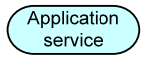
\includegraphics[scale=0.36,]{imagenes/lenguaje/Aplication/serviceApp}}
		\\ \hline
	\end{tabular}
	\caption{Capa de Aplicación}
	\label{capaAplicacion}
\end{table}

\subsection{Resumen: capa de motivación}
\begin{table}[H]
	\centering
	\begin{tabular}{|p{3cm}|p{6cm}|p{5,5cm}|}
		\hline
		\textbf{Concepto} & \multicolumn{1}{c|}{\textbf{Definición}}                                                             & \textbf{Notación} \\ \hline
		
		\begin{tabular}[c]{@{}c@{}}
			\\Interesados \\ (Stakeholder)
		\end{tabular} 
		& El rol de un individuo, equipo u organización (o clases de ellos) que representa sus intereses o preocupaciones, relativas al resultado de la arquitectura.
		& \raisebox{-0.75\totalheight}{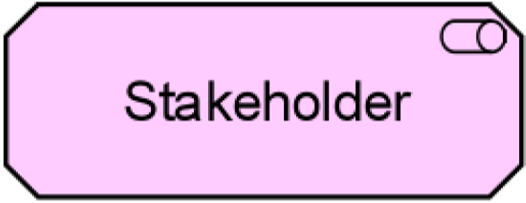
\includegraphics[scale=0.36,]			{imagenes/lenguaje/Motivational/stakeholder}}
		\\ \hline
		
		\begin{tabular}[c]{@{}c@{}}
			\\Conductor\\ (Driver)
		\end{tabular} 
		& Algo que crea, motiva y alimenta el cambio en una organización. 
		
		& \raisebox{-0,55\totalheight}{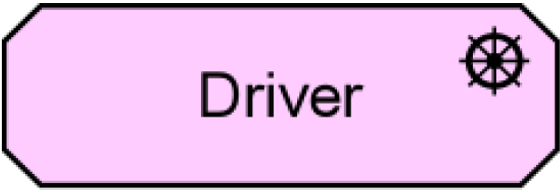
\includegraphics[scale=0.36,]			{imagenes/lenguaje/Motivational/driver}}
		\\ \hline
		
		\begin{tabular}[c]{@{}c@{}}
			\\Evaluación\\ (Assessment)
		\end{tabular}                  
		& El resultado de algunas evaluaciones de algunos conductores. 
		
		& \raisebox{-0,65\totalheight}{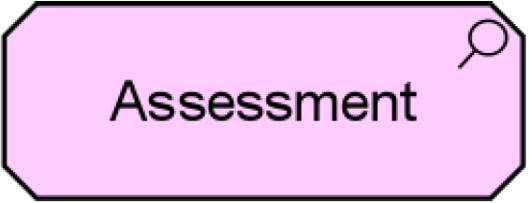
\includegraphics[scale=0.36,]			{imagenes/lenguaje/Motivational/assessment}}
		\\ \hline
		
		\begin{tabular}[c]{@{}c@{}}
			\\Gol\\ (Goal)
		\end{tabular}                      
		& Un estado final que una parte interesada desea lograr.    
		
		& \raisebox{-0,55\totalheight}{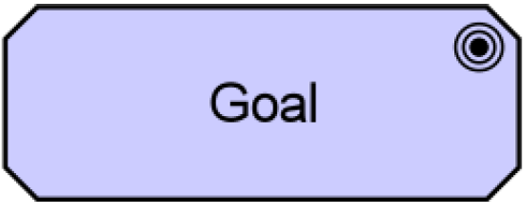
\includegraphics[scale=0.36,]			{imagenes/lenguaje/Motivational/goal}}
		\\ \hline
		
		\begin{tabular}[c]{@{}c@{}}
			\\Requisito\\ (Requirement)
		\end{tabular}                      
		&  Una declaración de necesidad que debe ser realizada por un sistema. 
		
		& \raisebox{-0,55\totalheight}{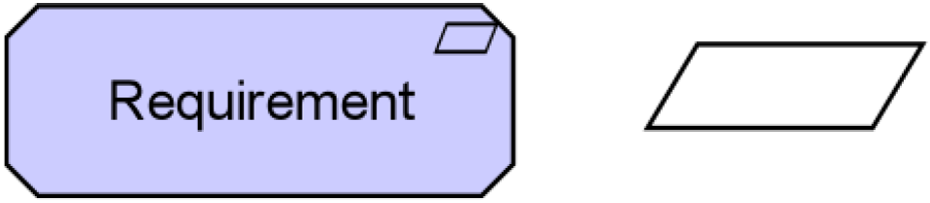
\includegraphics[scale=0.36,]			{imagenes/lenguaje/Motivational/requirement}}
		\\ \hline
		
		\begin{tabular}[c]{@{}c@{}}
			\\Restricción\\(Constraint)
		\end{tabular}                      
		& Una restricción de la forma en que se realiza un sistema.
		
		& \raisebox{-0,55\totalheight}{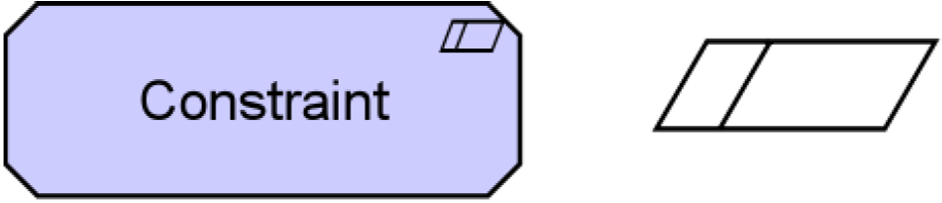
\includegraphics[scale=0.36,]			{imagenes/lenguaje/Motivational/constraint}}
		\\ \hline
		
		\begin{tabular}[c]{@{}c@{}}
			\\Principio\\ (Principle)
		\end{tabular}                      
		& Una propiedad normativa de todos los sistemas en un contexto dado, o la forma en que se realizan.                         
		& \raisebox{-0,66\totalheight}{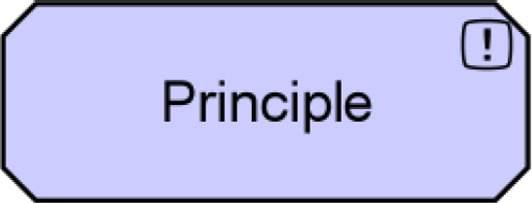
\includegraphics[scale=0.36,]			{imagenes/lenguaje/Motivational/principle}}
		\\ \hline
	\end{tabular}
	\caption{Capa de Motivación}
	\label{capaMotivacion}
\end{table}

\subsection{Resumen: capa de proyecto}
\begin{table}[H]
	
	\centering
	\begin{tabular}{|p{4cm}|p{5cm}|p{4cm}|}
		\hline
		\textbf{Concepto}                                                           & \multicolumn{1}{c|}{\textbf{Definición}}                                                             & \textbf{Notación} \\ \hline
		\begin{tabular}[c]{@{}c@{}}Paquete de Trabajo\\ (Work Package)\end{tabular} & Una serie de acciones diseñadas para lograr una meta única dentro de un tiempo especificado.         & 
		\raisebox{-\totalheight}{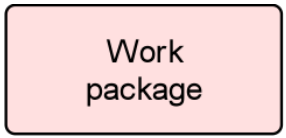
\includegraphics[scale=0.36,]			{imagenes/lenguaje/Proyect/WorkPackage.png}}
		\\ \hline
		\begin{tabular}[c]{@{}c@{}}Entregable\\ (Derivable)\end{tabular}            & Un resultado definido con precisión de un paquete de trabajo (work package).                         & 
		\raisebox{-\totalheight}{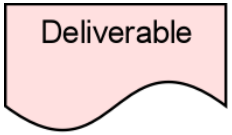
\includegraphics[scale=0.36,]			{imagenes/lenguaje/Proyect/Deliverable.png}}
		\\ \hline
		\begin{tabular}[c]{@{}c@{}}Meseta\\ (Plateau)\end{tabular}                  & Un estado relativamente estable de la arquitectura que existe durante un período de tiempo limitado. &  
		\raisebox{-\totalheight}{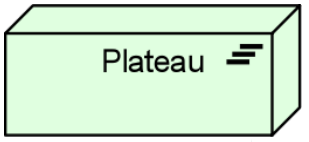
\includegraphics[scale=0.36,]			{imagenes/lenguaje/Proyect/Plateau.png}}
		\\ \hline
		\begin{tabular}[c]{@{}c@{}}Brecha\\ (Gap)\end{tabular}                      & Resultado de un análisis de la brecha entre dos mesetas (plateaus).                                  &  
		\raisebox{-\totalheight}{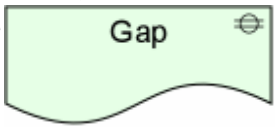
\includegraphics[scale=0.36,]			{imagenes/lenguaje/Proyect/Gap.png}}
		\\ \hline
	\end{tabular}
	\caption{Capa de Proyecto}
	\label{capa-proyecto}
\end{table}


\subsection{Resumen: capa de tecnologia}
\begin{center}
\begin{longtable}[H]{| >{\centering\arraybackslash}m{3cm} | >{\arraybackslash}m{6cm} | p{4cm} | p{5cm} | p{4cm} |}
	
		\hline
		\textbf{Concepto} &  \centering \textbf{Definición} & \textbf{Notación} \\
		\hline
		\endfirsthead
		
		
		\hline
		\textbf{Concepto} &  \centering \textbf{Definición} & \textbf{Notación} \\
		\hline
		\endhead
		
		Nodo        
		& \vspace{1mm} Un recurso computacional sobre el cual 
		los artefactos pueden ser almacenados o
		desplegados para su ejecución.        
		&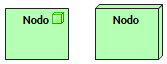
\includegraphics[width=30mm,trim=0 0 0 -2mm]{imagenes/lenguaje/tecnologia/nodo}  \\ \hline
		
		Dispositivo 
		& \vspace{1mm} Un recurso de hardware en el que los
		artefactos se pueden almacenar o desplegar 
		para su ejecución.              
		& 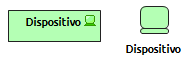
\includegraphics[width=35mm,trim=0 0 0 -2mm]{imagenes/lenguaje/tecnologia/dispositivo}  \\ \hline
		
		Red         
		&\vspace{1mm} Un medio de comunicación entre dos o
		más dispositivos.               
		& 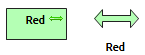
\includegraphics[width=25mm,trim=0 0 0 -2mm]{imagenes/lenguaje/tecnologia/red}  \\ \hline
		
		Ruta de 
		Comunicación	
		& \vspace{1mm} Un enlace entre dos o más nodos, a
		través del cual estos nodos pueden 
		intercambiar datos.                
		& 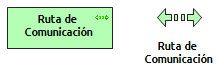
\includegraphics[width=35mm,trim=0 0 0 -2mm]{imagenes/lenguaje/tecnologia/comunicacion}  \\ \hline
		
		Interfaz de 
		infraestructura &\vspace{1mm} Un punto de acceso donde los servicios
		de infraestructura ofrecidos por un nodo 
		pueden ser accedidos por otros nodos y 
		componentes de la aplicación.
		&  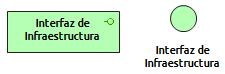
\includegraphics[width=35mm,trim=0 0 0 -2mm]{imagenes/lenguaje/tecnologia/interfaz}  \\ \hline
		
		Software del  
		Sistema
		&\vspace{1mm} Un entorno de software para tipos específicos de componentes y objetos que
		se despliegan en él en forma de artefactos.
		& 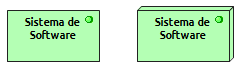
\includegraphics[width=35mm,trim=0 0 0 -2mm]{imagenes/lenguaje/tecnologia/software}  \\ \hline 
		
		Función de 
		Infraestructura 
		&\vspace{1mm} Un elemento de comportamiento que agrupa el comportamiento de infraes
		tructura que puede ser realizado por un	nodo.
		& 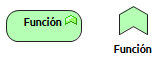
\includegraphics[width=35mm,trim=0 0 0 -2mm]{imagenes/lenguaje/tecnologia/funcion}  \\ \hline 	
		
		Servicio de 
		Infraestructura 
		&\vspace{1mm} Una unidad de funcionalidad visible externamente, proporcionada por uno o más nodos, expuesta a través de interfaces bien definidas y significativa para el entorno.
		&  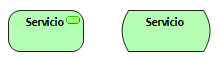
\includegraphics[width=35mm,trim=0 0 0 -2mm]{imagenes/lenguaje/tecnologia/servicio} \\ \hline 
		
		Artefacto 
		&\vspace{1mm} Una pieza física de datos que se utiliza ose produce en un proceso de desarrollo de software, o mediante el despliegue y la operación de un sistema. 
		& 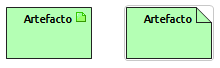
\includegraphics[width=35mm,trim=0 0 0 -2mm]{imagenes/lenguaje/tecnologia/artefacto}  \\ \hline
		

	\caption{Conceptos de Capa de Tecnología}
	
\end{longtable}
\end{center}


\subsection{Resumen Relaciones}

\subsubsection{Relaciones Estructurales}
\begin{center}
	\begin{longtable}[H]{| >{\centering\arraybackslash}m{3cm} | >{\arraybackslash}m{6cm} | p{4cm} | p{5cm} | p{4cm} |}
		
		\hline
		\textbf{Concepto} &  \centering \textbf{Definición} & \textbf{Notación} \\
		\hline
		\endfirsthead
		
		
		\hline
		\textbf{Concepto} &  \centering \textbf{Definición} & \textbf{Notación} \\
		\hline
		\endhead
		
		Asociacion       
		& \vspace{1mm} La asociación modela una relación entre
		objetos que no están cubiertos por otra más
		relación específica.        
		&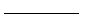
\includegraphics[width=30mm,trim=0 0 0 -2mm]{imagenes/lenguaje/relaciones/asociacion}  \\ \hline
		
		Acceso
		& \vspace{1mm} La relación de acceso modela el acceso de
		Conceptos conductuales para negocios o datos
		objetos.            
		& 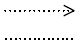
\includegraphics[width=35mm,trim=0 0 0 -2mm]{imagenes/lenguaje/relaciones/acceso}  \\ \hline
		
		Usado por        
		&\vspace{1mm} El utilizado por la relación modela el uso de
		servicios por procesos, funciones o
		interacciones y el acceso a las interfaces por
		roles, componentes o colaboraciones.               
		& 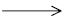
\includegraphics[width=25mm,trim=0 0 0 -2mm]{imagenes/lenguaje/relaciones/usadopor}  \\ \hline
		
		Realización	
		& \vspace{1mm} La relación de realización vincula una lógica
		entidad con una entidad más concreta que
		se da cuenta.              
		& 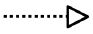
\includegraphics[width=35mm,trim=0 0 0 -2mm]{imagenes/lenguaje/relaciones/realizacion}  \\ \hline
		
		Asignación &\vspace{1mm} La relación de asignación vincula unidades de
		comportamiento con elementos activos (por ejemplo, roles,
		componentes) que los realizan, o roles con
		actores que los cumplen. 
		&  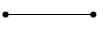
\includegraphics[width=35mm,trim=0 0 0 -2mm]{imagenes/lenguaje/relaciones/asignacion}  \\ \hline
		
		Agregacion
		&\vspace{1mm}  La relación de agregación indica que un
		el objeto agrupa varios otros objetos.
		& \includegraphics[width=35mm,trim=0 0 0 -2mm]{imagenes/lenguaje/relaciones/agregacion}  \\ \hline 
		
		Composición 
		&\vspace{1mm} La relación de composición indica que
		un objeto se compone de uno o más
		objetos.
		& \includegraphics[width=35mm,trim=0 0 0 -2mm]{imagenes/lenguaje/relaciones/composicion}  \\ \hline 			
		
		\caption{Conceptos de Capa de Relaciones Estructurales}
		
	\end{longtable}
\end{center}

\subsubsection{Relaciones Dinámicas}
\begin{center}
	\begin{longtable}[H]{| >{\centering\arraybackslash}m{3cm} | >{\arraybackslash}m{6cm} | p{4cm} | p{5cm} | p{4cm} |}
		
		\hline
		\textbf{Concepto} &  \centering \textbf{Definición} & \textbf{Notación} \\
		\hline
		\endfirsthead
		
		
		\hline
		\textbf{Concepto} &  \centering \textbf{Definición} & \textbf{Notación} \\
		\hline
		\endhead
		
		Flujo      
		& \vspace{1mm} La relación de flujo describe el intercambio
		o transferencia de, por ejemplo, información o
		valor entre procesos, función,
		interacciones y eventos.       
		&\includegraphics[width=30mm,trim=0 0 0 -2mm]{imagenes/lenguaje/relaciones/flujo}  \\ \hline
		
		Desencadenante
		& \vspace{1mm} La relación de activación describe el
		relaciones temporales o causales entre
		procesos, funciones, interacciones y eventos.  
		& \includegraphics[width=35mm,trim=0 0 0 -2mm]{imagenes/lenguaje/relaciones/triggering}  \\ \hline
		
		\caption{Conceptos de Capa de Relaciones Dinámicas}
		
	\end{longtable}
\end{center}

\subsubsection{Otras Relaciones}
\begin{center}
	\begin{longtable}[H]{| >{\centering\arraybackslash}m{3cm} | >{\arraybackslash}m{6cm} | p{4cm} | p{5cm} | p{4cm} |}
		
		\hline
		\textbf{Concepto} &  \centering \textbf{Definición} & \textbf{Notación} \\
		\hline
		\endfirsthead
		
		
		\hline
		\textbf{Concepto} &  \centering \textbf{Definición} & \textbf{Notación} \\
		\hline
		\endhead
		
		Agrupamiento     
		& \vspace{1mm} La relación de agrupamiento indica que
		objetos del mismo tipo o tipos diferentes
		pertenecen juntos basados en algunos
		característica.   
		&\includegraphics[width=15mm,trim=0 0 0 -2mm]{imagenes/lenguaje/relaciones/agrupacion}  \\ \hline
		
		Union
		& \vspace{1mm} Un cruce se usa para conectar relaciones de
		el mismo tipo
		& \includegraphics[width=10mm,trim=0 0 0 -2mm]{imagenes/lenguaje/relaciones/union}  \\ \hline
		
		
		
		Especialización
		& \vspace{1mm}La relación de especialización indica que
		un objeto es una especialización de otro objeto.
		& \includegraphics[width=35mm,trim=0 0 0 -2mm]{imagenes/lenguaje/relaciones/especializacion}  \\ \hline
		
		
		\caption{Conceptos de Capa de Relaciones Dinámicas}
		
	\end{longtable}
\end{center}
